% this file is called up by thesis.tex
% content in this file will be fed into the main document

%: ----------------------- name of chapter  -------------------------
\chapter{Background}\label{background} % top level followed by section, subsection


%: ----------------------- paths to graphics ------------------------

% change according to folder and file names
%\graphicspath{{2-Consorzi/images/}}


%: ----------------------- contents from here ------------------------
To fully understand how M2MShare works and what kind of simulator have to be used to emulate it, is worth to take a look at some technology backgrounds which can be useful to know before go further to the following of the thesis. In this chapter we describe what a DTN is, the notion of peer-to-peer and overlay networks.

\section{Delay\/Disruption Tolerant Networks (DTN)}
The Internet is a connected network where internet protocols, most notably transmission control protocol/internet protocol (TCP/IP), are dependent upon (low) latencies of approximately milliseconds. This low latency, coupled with low bit error rates, allows TCP to reliably transmit and receive acknowledgements for messages traversing the terrestrial Internet. 
\\

A DTN is a network designed to operate effectively in highly-challenged environments where protocols adopted in connected networks (i.e. TCP/IP) fail. The \"D\" part in DTN acronym stands both for \textit{Delay} and for \textit{Disruption}. By delay we mean the end-to-end latency of data transmission. Some of those delays are inherent in the transmission medium, or the geometry of the system, but others are due to packets being temporarily stored on intermediate nodes. By disruption, we mean factors that cause connections to break down, or not be established, normally due to transient or quickly changing aspects of the system and/or its environment.
\\

There are some environments where low latency and end-to-end links are rarely available. One of the best examples of high latency with intermittent connectivity is that of space communications \cite{Burleigh2003365}. One-way trip times, at the speed of light, from the Earth to the Moon incurs a delay of 1.7 seconds; while one-way trip times to Mars incur a minimum delay of 8 minutes. The problem of latency for interplanetary links is exasperated with increased error rate due to solar radiation. In addition, the celestial bodies are in constant motion, which can block the required line-of-sight between transmit and receive antennas, resulting in links that at best are only intermittently connected. 
\\

DTNs need not be solely concerned with deep-space communications but can also be useful in terrestrial networks. In some environment, networks may be subjected to high disruption probability. One example is military application, where adopting DTNs allows the retrieval of critical information in mobile battlefield scenarios using only intermittently connected network communications. Another application, more peaceful, is the adoption of DTNs to overcome a major natural disaster. In such a situation terrestrial infrastructures may have been swept away and tolerant protocols must be used to coordinate rescue teams.  
\\
Networks adopted in these situations are characterized by:
\begin{itemize}
\item \textbf{Intermittent Connectivity:} if there is no end-to-end path between source and destination, end-to-end communication using the TCP/IP protocols does not work.
\item \textbf{Long or Variable Delay:} in addition to intermittent connectivity, long propagation delays between nodes and variable queuing delays at nodes contribute to end-to-end path delays that can defeat Internet protocols and applications that rely on quick return of acknowledgements or data.
\item \textbf{Asymmetric Data Rates:} the Internet supports moderate asymmetries of bidirectional data rate for users with cable TV or asymmetric DSL access. But if asymmetries are large, they defeat conversational protocols.
\item \textbf{High Error Rates:} bit errors on links require correction (which requires more bits and more processing) or retransmission of the entire packet (which results in more network traffic). For a given link-error rate, fewer retransmissions are needed for hop-by-hop than for end-to-end retransmission.
\end{itemize}

To overcome problems associated with all these factors, DTNs use a old yet affective method used in postal systems since ancient times. In this method, named \textit{Store-and-forwarding}, node physically delivers data to the destination moving from the source location to the destination of the recipient node (\figurename~\ref{fig:store-carry-forward}). Replication techniques can be adopted to increase the deliver ratio, copying the carried data and giving it to other nodes following a different physical path.

\begin{figure}[htpb]
  \begin{center}
    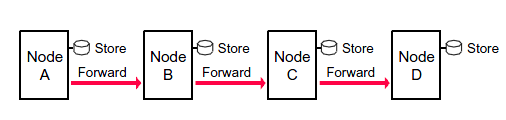
\includegraphics[scale=0.6]{2-background/img/store-and-forward.png}
    \caption{\textit{Store-and-forwarding} technique example}    
    \label{fig:store-carry-forward}
  \end{center}
\end{figure}

Messages are stored in storage mediums which can hold them for a long time period called persistent storage. This is another difference with internet protocols, where routers adopt very short-term storage provided by memory chips to store incoming packets. In Internet routers messages are queued only for a few milliseconds while they are waiting for their next hop. In DTNs routers need persistent storage for one or more of the following reasons:
\begin{itemize}
\item A communication link to the next hop may not be available for a long time and during this period message must be stored in the router.
\item There could be asymmetries in speed and reliability between nodes, so one node in a communicating pair may send or receive data much faster or more reliably than the other node.
\item A message, once transmitted, may need to be retransmitted if an error occurs at an upstream node or link, or if an upstream node declines acceptance of a forwarded message.
\item By moving whole messages in a single transfer, the message-switching technique provides network nodes with immediate knowledge of the size of messages, and therefore the requirements for intermediate storage space and retransmission bandwidth.
\end{itemize}





 
 
 


- Caratteristiche di una DTN 
   - Esempi di cause di Delay and Disruption
   - Inefficienza di protocolli classici su DTN ion caratteristiche
related work dtn mobile


\section{Related works}
% ---------------------------------------------------------------------------
%: ----------------------- end of thesis sub-document ------------------------
% ---------------------------------------------------------------------------

